\chapter{Pérdida de energía de iones en elementos pesados}

%%%%%%%%%%%%%%%%%%%%%%%%%%%%%%%%%%%%%%%%%%%%%%%%%%%%%%%%%%%%%%%%%%%%%%%%
\section{Introducción}
%%%%%%%%%%%%%%%%%%%%%%%%%%%%%%%%%%%%%%%%%%%%%%%%%%%%%%%%%%%%%%%%%%%%%%%%
\label{sec:intro}

El estudio de procesos de pérdida de energía por impacto de iones 
en sólidos es una poderosa herramienta en diversas áreas de la ciencia
básica y tecnología de materiales. Para energías de impacto superiores 
a unos pocos keV/amu, las partículas cargadas monoenergéticas que 
penetran algún material pierden su energía a través de una serie de 
colisiones inelásticas consecutivas, principalmente con blancos
electrónicos~\cite{Chu:01,Sigmund:06}. La información proporcionada por 
el proceso de pérdida de energía es esencial no solo para tener una 
mejor comprensión de la física detrás de las interacciones fundamentales, 
sino también porque juega un papel fundamental en muchos campos 
aplicados como la ciencia de materiales, la física nuclear, la 
implantación iónica y la radioterapia~\cite{Sigmund:06,Schardt:10}. 
Tablas y códigos resultantes de cálculos semiempíricos están disponibles 
para una gran combinación de iones y objetivos~\cite{iaea_codes,Paul:03}. 
Sin embargo, datos experimentales y predicciones teóricas 
\textit{ab initio} son de crucial importancia para comprobar la 
fiabilidad de los modelos semiempíricos y determinar ciertos 
parámetros clave~\cite{Diwan:15,Damache:04,Damache:02} para la pérdida 
de energía media de iones por trayecto unitario $S(E)$. Los datos 
experimentales disponibles son a menudo bastante escasos para materiales 
correspondientes a elementos de baja presencia en la corteza superior de 
la Tierra. Por otro lado, los cálculos de dispersión inelástica de 
blancos pesados a partir de métodos basados en primeros principios 
constituyen una difícil tarea ya que resulta necesario tener en cuenta 
efectos relativistas. Estos efectos son importantes no sólo para definir 
el estado de los electrones internos sino también para determinar las 
energías de ligadura de las capas externas.

En este capítulo, examinaremos la estructura atómica de blancos pesados
y el proceso de pérdida de energía de iones cuando inciden sobre ellos.
El método de Dirac--Fock (\acs{df}) es quizás la aproximación más 
conocida para el cálculo de funciones radiales y energías orbitales de 
átomos relativistas. Esta aproximación se basa en el principio 
variacional y puede producir resultados muy precisos. Sin embargo, el 
principio variacional presenta varios inconvenientes: el precio de la 
precisión del método se paga con funciones de onda radiales dependientes 
de los términos, las cuales no son ortogonales entre configuraciones. 
Estas características hacen que el uso de las funciones de onda sea 
engorroso en el cálculo las transiciones radiativas y de colisión. Más 
aún, dado que el principio variacional implica la minimización de la 
energía total, las energías de transición entre niveles cercanos se 
obtienen como diferencias muy pequeñas entre números grandes, y los 
resultados son muy susceptibles a errores numéricos. Esto es 
especialmente importante para los átomos pesados porque la energía total 
es muy grande. 

La aproximación teórica que se implementa aquí para describir los 
blancos relativistas fue desarrollada por Klapisch y colaboradores 
\cite{Klapisch:77,Koenig:72,Klapisch:71,Klapisch:67}. En este método, 
el Hamiltoniano multielectrónico de Dirac se resuelve a partir de la 
combinación de la teoría de perturbaciones y la aproximación de campo 
central. La ecuación de Dirac se resuelve y se obtienen las funciones 
de onda de orden cero. El Hamiltoniano resultante es luego diagonalizado 
en las bases de estas funciones implementando el método de interacción 
de configuraciones~(\acs{ci}). El término de Breit y los efectos 
electrodinámicos cuánticos (\acs{qed}) se incluyen a las energías como
correcciones de segundo orden. La descripción 
precisa de los blancos relativistas requiere la optimización de las 
configuraciones definidas; es necesario considerar solo aquellas que 
influyen de manera significativa en el CI. 
{\color{red} Poner algo sobre que el número de configuraciones es 
limitado porque sino todo se desmadra.} 
Las funciones de onda y energías relativistas obtenidas se implementan
luego para describir el blanco en el cálculo de pérdida de energía. La 
correcta descripción de blancos pesados que cuentan con electrones en la 
capa $4f$ es particularmente importante ya que estos electrones tiene un 
rol fundamental en la predicción de pérdida de energía a energías 
bajas~\cite{Roth:17}. 

El enfoque teórico considerado para el cálculo de pérdida de energía 
implementa la aproximación de plasma local por capa (\acs{slpa}) 
\cite{Montanari:13} para describir la energía transferida a los 
electrones ligados $1s$-$4f$ y dos modelos diferentes para el gas de 
electrones libre (\acs{feg}); en la región de baja energía, el modelo 
de potencial apantallado con condición de cúspide (\acs{spcc}) 
\cite{Montanari:17}, que está basado en un formalismo binario no lineal, 
y el formalismo dieléctrico de Mermin-Lindhard (\acs{dielectric-ml}) 
\cite{Mermin:70} para energías alrededor del frenado máximo y 
superiores. Este modelo requiere conocer las funciones de onda 
relativistas y energías de ligadura del blanco, considerando un cierto 
número de electrones de las capas externas en el FEG~\cite{Mendez:19}. 
% El hafnio es particularmente interesante ya que la subcapa 4f (con 14 electrones) es el principal contribuyente por debajo del FEG, lo que hace que las secciones eficaces de frenado sean muy sensibles a una buena descripción de esta capa. Se ha considerado el apantallamiento entre los electrones 4f y 5p y se ha descubierto que juega un papel importante en los cálculos de SLPA.

En este capítulo estudiaremos tres grupos de átomos de la tabla 
periódica: lantánidos con la capa $4f$ abierta (Gd y Er) y metales de 
transición pesados con la capa $4f$ completa (Hf y Pt). 
{\color{red} Escribir sobre las aplicaciones de los blancos que voy a 
tratar: Gd, Er, Hf y Pt  (ver paper de Moro).}

%So far, only one experimental work has been published regarding the stopping power cross section of pure hafnium for protons~\cite{Sirotinin}, while more attention has been recently given to studies involving hafnium oxide due to its practical use~\cite{Abril,Behar,Primetzhofer,Roth}. It is well known that significant attention has been paid in recent years to transition metal-oxides such as HfO$_2$ because of their potential as alternative gate dielectrics to replace SiO$_2$ for the future generation of nano-electronics with less than 45 nm gate length~\cite{Choi,Robertson}. Some important physical properties of the above mentioned metal-oxide films depend on their thickness, which is often measured by using Rutherford Backscattering Spectrometry~\cite{Alfassi01,Tesmer01}. This method relies on the determination of both the scattering cross section and also the stopping power of ion beams in the material of interest.

%In this study, we report experimental stopping power cross sections over the incident energy range (0.6-2.5) MeV for protons crossing self-supported Hf thin-film by using the transmission method. We aim not only to upgrade stopping power data compilations~\cite{HPaul03,mondim17} but also to provide useful information about the processes governing the slowing down of protons in multi-electronic targets. In the rare earth metals, the $4f$ electrons play an essential role in the stopping power since they belong to the first shell of bound electrons below the conduction band. As already noted \cite{Roth17}, the free electron gas (FEG) shows unexpected behavior in these elements, which casts doubts on its proper description. In the case of Hf, we found the contribution of the $4f$-shell to be decisive even at impact energies around the stopping maximum, as will be shown later.

Los detalles teóricos del cálculo de los blancos relativistas a estudiar 
se dan en la sección~\ref{sec:method-target}. Los modelos teóricos 
implementados para la predicción de la pérdida de energia se detallan en 
la sección~\ref{sec:method-stopping}. Los resultados de este trabajo se 
presentan en la sección~\ref{sec:results-heavy}. Las descripciones 
obtenidas para los blancos Gd, Er, Hf y Pt a partir de la 
resolución de la ecuación de Dirac en forma perturbativa se muestran y 
discuten en la sección~\ref{subsec:results-target}. 
Las energías de enlace resultantes se comparan con valores 
experimentales~\cite{Williams:95} y con la descripción dada por 
Desclaux mediante el método de Dirac--Fock~\cite{Desclaux:73}. 
Las predicciones de pérdida de energía obtenidas por nuestro modelo en 
los blancos pesados seleccionados se muestran y discuten la
sección~\ref{subsec:results-stopping}. Se realizan comparaciones con los 
modelos teóricos de Grande y Schiwietz~\cite{Grande:01,casp52}, y de 
Sigmund y Schinner~\cite{DPASS20}. Debido a su gran implementación en 
diversas aplicaciones, también se consideran los valores semi-empiricos 
dados por el paquete SRIM-2013~\cite{Ziegler01} y las tablas 
ICRU-49~\cite{ICRU49}. Las conclusiones de nuestro trabajo se encuentran 
al final del capítulo, en la sección~\ref{sec:conclu-heavy}.

%%%%%%%%%%%%%%%%%%%%%%%%%%%%%%%%%%%%%%%%%%%%%%%%%%%%%%%%%%%%%%%%%%%%%%%%
\section{Descripción de blancos relativistas}
%%%%%%%%%%%%%%%%%%%%%%%%%%%%%%%%%%%%%%%%%%%%%%%%%%%%%%%%%%%%%%%%%%%%%%%%
\label{sec:method-target}

La descripción de los estados de átomos pesados relativistas se 
obtiene resolviendo el Hamiltoniano multielectrónico de 
Dirac~\cite{Klapisch:77,Koenig:72,Klapisch:71,Klapisch:67}
\begin{equation}
 H = H' + H_{\mathrm{\mbox{\scriptsize Breit}}}(i,j) +
 H_{\mbox{\scriptsize QED}}\,,
\label{eq:htot}
\end{equation}
donde $H_{\mathrm{\mbox{\scriptsize Breit}}}(i,j)$ es el término de 
Breit, $H_{\mbox{\scriptsize QED}}$ considera los efectos 
electrodinámicos cuánticos (\acs{qed}), y
\begin{equation}
 H' = \sum_i \left[ h_i^{\mbox{\scriptsize D}} - \frac{Z}{r_i}\right]
 + \sum_{i<j}\frac{1}{r_{ij}}\,,
\label{eq:HDirac}
\end{equation}
siendo $h_i^{\mbox{\scriptsize D}}$ el término cinético del 
Hamiltoniano de Dirac de una partícula. Los términos restantes en la
ecuación~(\ref{eq:hprim}) corresponden a las interacciones 
núcleo--electrón y electrón--electrón, respectivamente. Usando la 
aproximación de campo central y mediante la introducción de un potencial 
paramétrico $U(\boldsymbol{\alpha},r)$, el Hamiltoniano $H'$ se puede escribir como la 
combinación de un término de orden cero, 
\begin{equation}
 H_0 = \sum_i h_i^{\mbox{\scriptsize D}} + U(\boldsymbol{\alpha},r_i)\,,
\end{equation}
más una pequeña perturbación
\begin{equation}
 H_1 = \sum_{i<j}\frac{1}{r_{ij}}
 - \sum_i \left[ \frac{Z}{r_i} + U(\boldsymbol{\alpha},r_i) \right]\,.
\end{equation}
Las soluciones de espinor de cuatro componentes de un electrón de la 
ecuación de Dirac
\begin{equation}
\left[ h_i^{\mbox{\scriptsize D}} +U(\boldsymbol{\alpha},r) \right] \varphi_{nljm}(\mathbf{r}) 
= \varepsilon_{nljm} \varphi_{nljm}(\mathbf{r})\,,
\label{eq:ecuacionDirac}
\end{equation}
llamadas orbitales relativistas, pueden ser caracterizadas por un 
conjunto de números cuánticos $nljm$, donde $l$ es el número cuántico 
del momento angular orbital de las componentes superiores. 
% componentes superiores = upper components ???

La solución de orden cero de un sistema $N$--electrónico se construye a 
partir de productos antisimetrizados de orbitales en cualquier esquema 
de acoplamiento elegido $\Gamma JM$ como 
\begin{equation}
\Psi_{\Gamma}\left(\mathbf{r}_1, \mathbf{r}_2, \ldots, \mathbf{r}_N\right)=A \sum_{all\,\,m}\left\langle\Gamma J M \mid m_1 m_2, \ldots, m_{N}\right\rangle \prod_{a} \varphi_{n_a l_a j_a m_a}\left(\mathbf{r}_a\right)\,,
\end{equation}
donde $A$ es el operador de antisimetría. Los estados y niveles 
específicos se denotan $\Gamma_iJ_iM_i$ y $\Gamma_iJ_i$, respectivamente,
donde $\Gamma_i$ representa el conjunto de números cuánticos necesario 
para identificar el estado de manera únivoca. 

Una configuración 
$C\equiv\prod_{a=1}^N\mathbf{j}_a=\prod_{i=1}\mathbf{j}_i^{q_i}$ es un 
conjunto de estados degenerados, con valores fijos $\mathbf{j}_i=n_il_ij_i$
y números de ocupación $q_i$, todos con energías de orden cero 
$E_C^0=\prod_{i=1}\,q_i\varepsilon_i$. 
El Hamiltoniano $H'$ se construye sobre la base de las configuraciones 
elegidas obtenidas con el potencial paramétrico. Luego, la matriz es 
diagonalizada, produciendo estados de configuración mixtos y energías 
de primer orden con algunas correcciones de correlación. Las funciones 
de onda resultantes se utilizan para agregar las correcciones QED y el 
término de Breit a las energías como perturbaciones de segundo orden.

La idea detrás del potencial paramétrico $U(\boldsymbol{\alpha},r)$ es 
describir de manera simple el apantallamiento de la distribución de carga 
de los electrones usando una expresión paramétrica analítica, donde 
$\boldsymbol{\alpha}=\left\{\alpha_1,\alpha_2,\ldots,\alpha_k\right\}$ 
es un conjunto de parámetros que se definen mediante la optimización 
del sistema y $k$ es el número de capas ocupadas. Aplicando la ecuación de 
Poisson a la densidad de carga radial de los $q$ electrones descritos 
por los orbitales de tipo Slater
\begin{equation}
\rho(r) = -4\pi r^2 qN\left|r^{l+1}e^{-\alpha r/2}\right|^2\,,
\end{equation} 
con las condiciones de borde 
\begin{equation}
U(\boldsymbol{\alpha},r\rightarrow\infty)=Z-\frac{q}{r}\,.
\end{equation} 
Aquí, $N$ es un factor de normalización, y $\alpha_i$ está relacionado 
con el radio medio de la capa tal que $\alpha_i=(2l+3)/\langle r\rangle_i$. 
Es necesario mostrar que el potencial para diversas capas y el nucleo 
se puede escribir como
\begin{equation}
U(\boldsymbol{\alpha},r)=-\frac{1}{r} \left[I+\sum_s q_s\, g(L_s,\alpha_s,r) 
+ \sum_t q_t\,f(l_t,\alpha_t,r)\right]\,,
\label{eq:potparam}
\end{equation}
donde los índices $s$ y $t$ recorren las capas cerradas y abiertas, 
respectivamente. El valor $I$ es el grado de ionización más uno. 
%Esto elimina la auto-interacción adicional de los electrones ligados. Aquí, $\boldsymbol{\alpha}$ representa un conjunto de parámetros $\left\{\alpha_s,\alpha_t\right\}$ que describen el radio medio de las capas. 
Las funciones $f$ y $g$ son tales que
\begin{eqnarray}
f(l,\alpha,r)&=&\mathrm{e}^{-\alpha r} \sum_{j=1}^{2 l+1}\left(1-\frac{j}{2 l+2}\right) \frac{(\alpha r)^{j}}{j !}\,, \\
g(L, \alpha, r)&=&\frac{1}{2 n^{2}} \sum_{l=0}^{L=n-1}(4 l+2) f\left(l, \alpha^{(l)}, r\right)\,,
\end{eqnarray}
donde $n$ es el número cuántico principal y $\alpha^{(l)}$ incluye una
corrección para la ligera diferencia en el radio debido al número del
momento angular cuántico de las subcapas. 
Los parámetros libres $q$ son el número efectivo de electrones en la 
capa y satisfacen $I+\sum_{s} q_{s}+\sum_{t} q_{t}=Z$. 

Esta parametrización resulta en que cualquier cantidad atómica calculada 
con las funciones de onda dadas por la ecuación~(\ref{eq:ecuacionDirac}) 
junto con el potencial~(\ref{eq:potparam}) se convierte en una función 
numérica de los parámetros. Hay múltiples formas posibles de elegir los 
parámetros $\boldsymbol{\alpha}$, de acuerdo a diversos criterios 
teóricamente válidos. Entre ellos, podemos nombrar tres;
\begin{itemize}
\item criterio espectroscópico: minimización de la desviación \acs{rms} 
entre los niveles de energía teóricos y experimentales,
\item criterio variacional: minimización de la energía total, y
\item criterio perturbacional: minimización del Hamiltoniano perturbativo
$H_1$. 
\end{itemize}
En nuestro trabajo, implementamos la minimización de las energías de 
configuración promedio (\acs{ca}), o de las energías de cualquier 
conjunto de niveles elegido. Dado que las energías de primer orden sobre 
las que actúa la optimización incluyen la contribución de intercambio 
exacta, los parámetros resultantes absorben el efecto del intercambio y, 
por lo tanto, no hay necesidad de un potencial de intercambio adicional 
explícito.

%la optimización de los blancos se realiza resoviendo la ecuación de Dirac a primer orden,

Por otro lado, siendo $U(\boldsymbol{\alpha},r)$ un potencial central,
es posible plantear la separación de variables esféricas de las 
soluciones de la ecuación de Dirac~(\ref{eq:ecuacionDirac}), tal que
\begin{equation}
\varphi_{nljm}(\mathbf{r}) = \frac{1}{r} \left( 
\begin{array}{c}
i P_{nlj}(r) \,\Omega_{jlm}(\hat{\mathbf{r}}) \\ 
  Q_{nlj}(r) \,(\boldsymbol{\sigma}\cdot\hat{\mathbf{r}})\,\Omega_{jlm}(\hat{\mathbf{r}})
\end{array}
\right)\,,
\label{eq:sepespinor}
\end{equation}
donde $P_{nlj}(r)$ y $Q_{nlj}(r)$ son los componentes fuerte y débil de los 
espinores de Dirac, respectivamente. Los espinores esféricos 
$\Omega_{jlm}(\hat{\mathbf{r}})$ son autoestados de $J^2$ y $J_z$ a 
través de la relación
\begin{equation}
\Omega_{j, l, m}(\theta, \phi)=\sum_{\mu} C(l, 1 / 2, j ; m-\mu, \mu, m) Y_{l, m-\mu}(\theta, \phi) \chi_{\mu}\,,
\end{equation}
donde $C\left(j_{1}, j_{2}, j ; m_{1}, m_{2}, m\right)$ son los
coeficientes de Clebsch--Gordan. Así, el valor esperado de cualquier 
operador $\hat{A}$ estará dado por
\begin{equation}
\langle\hat{A}\rangle=\int_0^{\infty}\left[P^*(r)\,\hat{A}\,P(r) 
 +Q^*(r)\,\hat{A}\,Q(r)
\right]\,dr\,.
\label{eq:meanvalr}
\end{equation}
Para los orbitales relativistas, usamos la notación $nl\pm$, que 
significa $nlj$, donde el índice $j=l\pm1/2$ se representa como $\pm$.

%%%%%%%%%%%%%%%%%%%%%%%%%%%%%%%%%%%%%%%%%%%%%%%%%%%%%%%%%%%%%%%%%%%%%%%%
\section{Modelo teórico de pérdida de energía}
%%%%%%%%%%%%%%%%%%%%%%%%%%%%%%%%%%%%%%%%%%%%%%%%%%%%%%%%%%%%%%%%%%%%%%%%
\label{sec:method-stopping}

La pérdida de energía de iones en blancos metálicos responde a diferentes
mecanismos físicos, dependiendo de la velocidad del proyectil incidente.
A bajas velocidades, las colisiones binarias son responsables de la 
pérdida de energía. La contribución principal es la ionización de los 
electrones de la banda de conducción del metal, que está aproximada por 
un gas de electrones libres (FEG) de velocidad de Fermi $v_F$. Por arriba
de un valor particular de velocidad (i.e., $v\geq 1.5\,v_F$), no solo 
ocurren excitaciones binarias sino también colectivas (plasmones) 
\cite{Montanari:17}. Más aún, a altas energías, los electrones ligados
también contribuyen al potencial de frenado. El método teórico de 
pérdida de energía combina una descripción de FEG para la interacción del
proyectil con los electrones de valencia (o conducción) y una 
aproximación diferente para la interacción con los electrones ligados.

Usamos el modelo de potencial apantallado con condición de cúspide 
(\acs{spcc})~\cite{Montanari:17} para describir el potencial de frenado 
de partículas cargadas con bajas velocidades de impacto en el FEG. Este 
método está basado en la aproximación de colisión binaria no 
perturbativa, de manera que es válida para valores de energías menores a 
las excitaciones de plasmones. La SPCC está basada en un potencial 
centrado apantallado con una condición de cúspide para la densidad 
electrónica cerca del proyectil. Este modelo ha probado dar buenas 
descripciones para la densidad de electrones inducida, aún para 
proyectiles con carga negativa. Además, este modelo predice correctamente 
las diferencias entre protón-antiprotón en el potencial de frenado, más 
conocido como el efecto Barkas. El formalismo SPCC depende sólo del radio 
de Wigner-Seitz $r_S$, que es una medida de la densidad electrónica del 
FEG. Para metales de $r_S$ conocidos, el SPCC describe correctamente los 
valores experimentales del potencial de frenado a bajas energías, en 
concordancia con resultados DFT de Echenique y 
colaboradores~\cite{Echenique:81,Nagy:89} a $v=0$.

Por encima de cierta velocidad de impacto, la contribución del plasmón 
es esencial (alrededor del máximo de la sección eficaz de frenado). Un 
valor de interés para nuestro análisis es la velocidad de impacto mínima 
para excitar plasmones, $v_P$. En el formalismo dieléctrico, este valor 
se puede obtener como $v_P\,\approx\,v_F[1+(3\pi\,v_F)^{-1/2}]$
\cite{suppression}. Para describir la pérdida de energía considerando la 
excitación colectiva y binaria, se recurre al formalismo dieléctrico de 
Mermin-Lindhard (ML)~\cite{Mermin:70}, que es una aproximación 
perturbativa de respuesta lineal, por lo que depende del cuadrado de la 
carga del proyectil. En este formalismo, la respuesta de los electrones 
del blanco al paso de iones se describe a través de la función 
dieléctrica cuántica, que depende de los parámetros característicos 
$r_S$ y $\delta$ del FEG.

La potencia de frenado debido a los electrones ligados se obtiene 
empleando la aproximación de plasma local por capa 
(SLPA)~\cite{Montanari:17,Montanari:13}. Vale la pena destacar que las 
únicas cantidades de las cuales depende este modelo son las densidades 
radiales orbitales del estado fundamental y sus energías de enlace. El 
modelo incluye los procesos colectivos y el apantallamiento entre 
electrones. 

Para la contribución de los electrones ligados a la sección eficaz de 
frenado total, el método de SLPA considera las contribuciones 
independientes de cada subcapa. Nuestras energías de ligadura 
relativistas presentan un desdoblamiento de espín-órbita. Sin embargo, 
en la potencia de frenado total, donde el estado inicial del electrón 
excitado no es medido, la incertidumbre cuántica en energía $\Delta E$ 
fusiona el desdoblamiento. El criterio $\Delta E\Delta t\geq\hbar/2$ une 
las energías $E_{nl+}-E_{nl-}$ para valores de tiempos medios de colisión
$\Delta t$ lo suficientemente pequeños. De hecho, a una velocidad de 
impacto suficientemente alta, podemos esperar que todos los electrones 
del blanco respondan juntos al paso de los 
iones~\cite{Lindhard:53,Chu:72}. Siguiendo trabajos 
previos~\cite{Montanari:09}, el tiempo de colisión se estima como 
$\Delta t\approx\langle r_i\rangle/v$, siendo $\langle r_i\rangle$ y $v$ 
el radio orbital medio y la velocidad de impacto, respectivamente. 
%En el caso del hafnio, encontramos que para cada subcapa de electrones, la división espín-órbita no se resuelve en la región de energía a la que contribuye esta subcapa. Por lo tanto, los nl-electrones deben considerarse juntos, respondiendo al paso de iones como un solo gas de electrones con densidad $\delta_{nl}(r)$ y energía de enlace media $E_{nl}$. Esta característica es vital dentro de los cálculos de SLPA porque explica el filtrado entre electrones de la misma energía de enlace.

%%%%%%%%%%%%%%%%%%%%%%%%%%%%%%%%%%%%%%%%%%%%%%%%%%%%%%%%%%%%%%%%%%%%%%%%
\section{Resultados}
%%%%%%%%%%%%%%%%%%%%%%%%%%%%%%%%%%%%%%%%%%%%%%%%%%%%%%%%%%%%%%%%%%%%%%%%
\label{sec:results-heavy}

En esta sección presentamos los resultados obtenidos de la optimización
de ciertos blancos relativistas y su implementación en el estudio de 
procesos de pérdida de energía tales como la potencia de frenado y la 
ionización de electrones de la capa $L$.

%%%%%%%%%%%%%%%%%%%%%%%%%%%%%%%%%%%%%%%%%%%%%%%%%%%%%%%%%%%%%%%%%%%%%%%%
\subsection{Energías de ligadura y valores medios}
%%%%%%%%%%%%%%%%%%%%%%%%%%%%%%%%%%%%%%%%%%%%%%%%%%%%%%%%%%%%%%%%%%%%%%%%
\label{subsec:results-target}

Los efectos de la interacción de configuraciones (\acs{ci}) son muy 
importantes en el caso de los átomos relativistas. Así, la correcta 
descripción del blanco depende de las configuraciones consideradas en 
el CI. En esta sección, la optimización de los blancos consiste en la 
determinación de las configuraciones que contribuyen de manera 
significativa a la mezcla en la interacción de configuraciones. 

El Hamiltoniano perturbativo de Dirac, dado por la 
ecuación~(\ref{eq:HDirac}), de los blancos relativistas a describir se 
resuelve aplicando el método perturbativo descrito anteriormente. Por 
simplicidad, llamamos a este método Dirac perturbativo (PD). Las 
soluciones numéricas se obtienen usando el paquete de códigos 
{\sc hullac}~\cite{BarShalom:01}. En este conjunto de programas 
computacionales, el código {\sc relac} permite calcular las energías 
relativistas y funciones de onda orbitales en primer orden. 

\begin{table*}[t]
\centering
\begin{tabular}{|c|c|c|c|l|}
\hline
Nombre   & Símbolo & $Z$ & Config. fundamental & Serie \\
\hline
\hline
Gadolinio & Gd & 64 & [Xe]~$4f^7\,5d\,6s^2$ & \multirow{2}{*}{Lantánidos} \\
Erbio     & Er & 68 & [Xe]~$4f^{12}\,6s^2$ & \\
\hline
Hafnio  & Hf & 72 & [Xe]~$4f^{14}\,5d^2\,6s^2$ & \multirow{2}{*}{Metales de transición}\\
Platino & Pt & 78 & [Xe]~$4f^{14}\,5d^9\,6s$ & \\
\hline
\end{tabular}
\caption[Blancos relativistas y sus configuraciones fundamentales]
{Blancos relativistas: símbolos, cargas nucleares $Z$, configuraciones 
fundamentales y serie.}
\label{tab:gruposrelat} 
\end{table*}

Los elementos que examinamos en esta sección se dividen en dos grupos 
según la serie de la tabla periódica a la que pertenecen. Los blancos a 
estudiar, sus símbolos, carga nuclear $Z$ y configuraciones fundamentales 
se muestran en la tabla~\ref{tab:gruposrelat}. El grupo de lantánidos a
analizar está compuesto por Gd y Er. Los metales de transición Hf y Pt 
conforman el grupo de metales de transición bajo estudio. 

Podemos escribir una fórmula general para la configuración fundamental 
de los lantánidos,
\begin{equation}
nf^w\,(n+1)d^x\,(n+2)s^y\,,
\end{equation}
donde $n=4$, $w=7,12$, $x=1,0$ y $y=2,2$. En el caso de Gd, también 
tenemos que incluir las interacciones entre los electrones de las capas
$4f$ y $5d$, que están abiertas. Así, las contribuciones más 
importantes a la interacción de configuraciones están dadas por la 
mezcla de las configuraciones $4f^7\,5d\,6s^2$ y $4f^8\,6s^2$.
Para Er, la mayor mezcla es producida por las configuraciones 
$4f^{12}\,6s^2$ y $4f^{12}\,5d\,6s$.

Por otro lado, podemos escribir la configuración fundamental de los 
metales de transición en forma general como
\begin{equation}
nd^w\,(n+1)s^x\,,
\end{equation}
donde $n=5$, $w=2,9$, $x=2,1$ para el grupo A. Los electrones $nd$ y 
$(n+1)s$ tienen energías de ligadura similares. Por lo tanto, las 
configuraciones 
\begin{gather}
nd^w(n+1)s^2, \\
nd^{w+1}(n+1)s, \\
nd^{w+2}
\end{gather}
tienen energías comparables. Dado que estas configuraciones tienen la 
misma paridad, éstas cumplen los dos requerimientos mencionados 
anteriormente, y son fundamentales en los cálculos de mezcla de 
configuraciones. Entonces, por ejemplo, para el átomo de Pt, las 
configuraciones [Xe]~$5d^9\,6s$ y $5d^{10}$ son consideradas en el 
cálculo relativista.

%%%%%%%%%%%%%%%%%%%%%%%%%%%%%%%%%%%%%%%%%%%%%%%%%%%%%%%%%%%%%%%%%%%%%%%%
Las energías de ligadura de los blancos relativistas de la 
tabla~\ref{tab:gruposrelat} que se obtienen a partir del método PD se 
dan en la tabla~\ref{tab:relatresults} y se muestran en la 
figura~\ref{fig:bindener} con diamantes rellenos. En la tabla se 
incluyen los valores medios $\langle r\rangle$ de cada capa, los cuales 
se obtienen a partir de la ecuación~(\ref{eq:meanvalr}). Datos 
experimentales de los blancos en estado sólido~\cite{Williams:95} se 
presentan usando círculos vacíos. Los resultados obtenidos por 
Desclaux~\cite{Desclaux:73} mediante la implementación del método 
de Dirac--Fock se muestran en la figura con símbolos $\times$. También 
se incluyen resultados no relativistas mediante la implementación del 
método de Hartree--Fock~\cite{FroeseFischer:97} con símbolos 
$\triangleleft$.

\begin{longtable}{|c|ccc|ccc|}
\caption[Energías de ligadura y valores $\langle r \rangle$ de blancos
relativistas]
{Energías de ligadura teóricas perturbativas y 
experimentales~\cite{Williams:95} de Gd, Er, Hf y Pt. 
Valores medios $\langle r \rangle$ en a.u. obtenidos a partir de la 
ecuación~(\ref{eq:meanvalr}).}
\label{tab:relatresults}\\
\hline
%% primer encabezado
\multirow{2}{*}{$nlj$} 
 & $E^{\mbox{\tiny exp}}$
 & $E^{\mbox{\tiny PD}}$
 & $\langle r\rangle^{\mbox{\tiny PD}}$
 & $E^{\mbox{\tiny exp}}$
 & $E^{\mbox{\tiny PD}}$
 & $\langle r\rangle^{\mbox{\tiny PD}}$ \\
\endfirsthead % fin de primer encabezado
%% segundo encabezado (tabla continuada)
\caption* {(Cont.): Energías de ligadura teóricas perturbativas y 
experimentales~\cite{Williams:95} de Gd, Er, Hf y Pt. 
Valores medios $\langle r \rangle$ en a.u. obtenidos a partir de la 
ecuación~(\ref{eq:meanvalr}).} \\
 \hline
$nlj$ 
 & $E^{\mbox{\tiny exp}}$
 & $E^{\mbox{\tiny PD}}$
 & $\langle r\rangle^{\mbox{\tiny PD}}$
 & $E^{\mbox{\tiny exp}}$
 & $E^{\mbox{\tiny PD}}$
 & $\langle r\rangle^{\mbox{\tiny PD}}$ \\
 \hline
\endhead
\hline
\endfoot
\endlastfoot
  \cline{2-7}
  &  \multicolumn{3}{c}{Gd}  &  \multicolumn{3}{c}{Er} \\
\hline
$1s$   & 1846.2 & 1843.6 & 0.0219 & 2112.7 & 2114.2 & 0.0203 \\
$2s$   & 307.8  & 303.0  & 0.0929 & 358.4  & 353.7  & 0.0858 \\
$2p_-$ & 291.4  & 287.2  & 0.0776 & 340.5  & 337.5  & 0.0712 \\
$2p_+$ & 266.2  & 261.6  & 0.0845 & 307.2  & 303.3  & 0.0785 \\
$3s$   & 69.13  & 67.43  & 0.244  & 81.07  & 79.34  & 0.225  \\
$3p_-$ & 62.03  & 60.79  & 0.234  & 73.72  & 72.00  & 0.215  \\
$3p_+$ & 56.74  & 55.50  & 0.247  & 66.59  & 64.92  & 0.229  \\
$3d_-$ & 44.904 & 44.084 & 0.219  & 53.40  & 51.91  & 0.202  \\
$3d_+$ & 43.717 & 42.953 & 0.223  & 51.78  & 50.38  & 0.207  \\
$4s$   & 13.91  & 13.50  & 0.553  & 16.53  & 15.62  & 0.507  \\
$4p_-$ & 10.5   & 10.9   & 0.565  & 13.46  & 12.69  & 0.515  \\
$4p_+$ & 9.96   & 9.74   & 0.596  & 11.77  & 11.06  & 0.548  \\
$4d_-$ & -      & 5.515  & 0.634  & 6.160  & 6.186  & 0.578  \\
$4d_+$ & 5.240  & 5.306  & 0.645  & 6.160  & 5.892  & 0.589  \\
$5s$   & 1.3    & 2.0    & 1.34   & 1.86   & 1.95   & 1.25   \\
$5p_-$ & 0.74   & 1.3    & 1.51   & 1.15   & 1.16   & 1.41   \\
$5p_+$ & 0.74   & 1.2    & 1.60   & 0.908  & 0.954  & 1.52   \\
$4f_-$ & 0.32   & 0.41   & 0.916  & -      & 0.18   & 0.813  \\
$4f_+$ & 0.32   & 0.38   & 0.934  & 0.17   & 0.14   & 0.838  \\
$6s$   &        & 0.31   & 3.70   &        & 0.19   & 4.33  \\
$5d_-$ &        & 0.29   & 2.50   &        &        &      \\
$5d_+$ &        & 0.28   & 2.56   &        &        &     \\
\hline
& \multicolumn{3}{c}{Hf} & \multicolumn{3}{c}{Pt} \\
\hline
$1s$   & 2401.6 & 2400.4 & 0.0190 & 2880.9 & 2881.6 & 0.0171 \\
$2s$   & 414.20 & 408.98 & 0.0798 & 510.08 & 504.78 & 0.0718 \\
$2p_-$ & 394.65 & 390.26 & 0.0662 & 487.77 & 483.25 & 0.0591 \\
$2p_+$ & 351.4  & 346.4  & 0.0740 & 424.97 & 419.70 & 0.0676 \\
$3s$   & 95.58  & 93.55  & 0.208 & 121.1  & 118.8  & 0.187 \\
$3p_-$ & 86.91  & 85.40  & 0.198 & 111.2  & 109.4  & 0.177 \\
$3p_+$ & 77.43  & 75.97  & 0.213 & 97.20  & 95.37  & 0.192 \\
$3d_-$ & 63.06  & 62.14  & 0.187 & 80.92  & 79.83  & 0.168 \\
$3d_+$ & 61.08  & 60.12  & 0.191 & 77.98  & 76.83  & 0.172 \\
$4s$   & 19.8   & 18.8   & 0.468 & 26.66  & 25.53  & 0.416 \\
$4p_-$ & 16.10  & 15.45  & 0.474 & 22.38  & 21.55  & 0.419 \\
$4p_+$ & 13.99  & 13.28  & 0.508 & 19.09  & 18.22  & 0.453 \\
$4d_-$ & 8.08   & 7.81   & 0.530 & 12.19  & 11.70  & 0.463 \\
$4d_+$ & 7.772  & 7.418  & 0.542 & 11.56  & 11.09  & 0.474 \\
$5s$   & 2.36   & 2.55   & 1.12  & 3.737  & 3.829  & 0.942 \\
$5p_-$ & 1.4    & 1.6    & 1.24  & 2.40   & 2.53   & 1.02 \\
$5p_+$ & 1.10   & 1.28   & 1.35  & 1.90   & 1.94   & 1.12 \\
$4f_-$ & 0.584  & 0.725  & 0.666 & 2.74   & 2.75   & 0.513 \\
$4f_+$ & 0.522  & 0.660  & 0.679 & 2.62   & 2.62   & 0.520 \\ 
$6s$   &        & 0.214  & 3.83  &        & 0.250  & 3.30 \\  
$5d_-$ &        & 0.125  & 2.77  &        & 0.250  & 1.71 \\  
$5d_+$ &        & 0.109  & 3.13  &        & 0.200  & 1.88 \\
\hline
\end{longtable}

\begin{figure}[H]
\centering
\includegraphics[width=\textwidth]{heavy/bindener.eps}
\caption[Energías de ligadura de blancos relativistas]
{Energías de ligadura de Gd, Er, Hf y Pt. Símbolos: 
$\blacklozenge$ resultados teóricos del presente trabajo, 
$\times$ valores teóricos del método Dirac--Fock~\cite{Desclaux:73}, 
$\triangleleft$ valores teóricos según Hartree--Fock, y 
$\medcircle$ datos experimentales en sólidos~\cite{Williams:95}.}
\label{fig:bindener}
\end{figure}

\begin{figure}[t]
\centering
\includegraphics[width=\textwidth]{heavy/ratios_heavy_barh.eps} 
%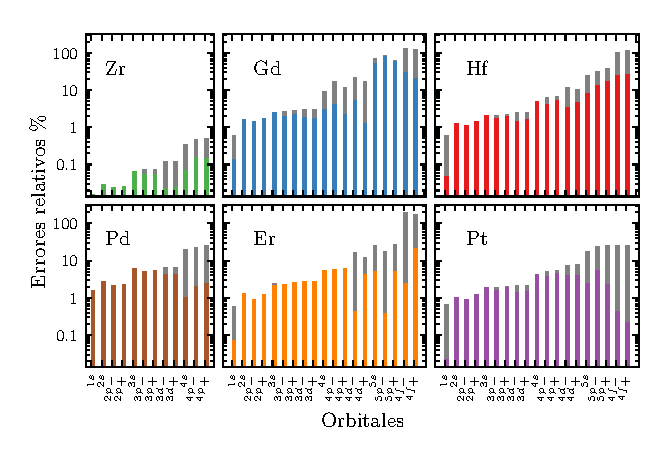
\includegraphics[width=\textwidth]{heavy/erp_heavy.eps} 
\caption[Razón $E^{\mbox{\scriptsize exp}}/E$ entre energías de ligadura 
experimentales y teóricas.]
{Razón $E^{\mbox{\scriptsize exp}}/E$ entre energías de ligadura 
experimentales y teóricas de Gd, Er, Hf y Pt: métodos de Hartree--Fock 
(barras gris oscuro), Dirac--Fock (barras gris claro), y Dirac 
perturbativo (barras de colores).}
\label{fig:ratios}
\end{figure}

Dado que la figura~\ref{fig:bindener} muestra las energías de enlace en 
un rango de magnitud de cinco órdenes, no es posible discernir las 
discrepancias entre los datos experimentales y los resultados teóricos
obtenidos mediante los métodos de Hatree--Fock, Dirac--Fock y Dirac 
perturbativo. Para poder inspeccionar estas diferencias con más detalle, 
las relaciones entre las energías de ligadura experimentales 
$E^{\mbox{\scriptsize exp}}$ y teóricas (HF, DF y PD) se muestran en la 
figura~\ref{fig:ratios}. La figura muestra claramente que las 
correcciones relativistas son críticas para describir la estructura 
atómica de los blancos considerados, incluso para las capas externas. 
Por ejemplo, la energía de enlace no relativista de la subcapa $4f$ de 
Hf es cuatro veces la experimental. Un valor tan incorrecto conduce a la 
subestimación de la ionización de los electrones $4f$ y desplaza el 
umbral a energías más altas. Por otro lado, los valores teóricos 
relativistas de Dirac--Fock mejoran la descripción de las capas internas 
de los blancos de forma sistemática. Sin embargo, las discrepancias con 
los valores experimentales en las capas cercanas a la banda de valencia 
son significativas. En definitiva, la incorrecta descripción de los 
orbitales de las capas internas se propaga a las capas externas en los 
cálculos no relativistas (HF) y relativistas (DF) que implementan el 
método variacional. 

En general, el acuerdo entre nuestros resultados teóricos perturbativos 
relativistas y las mediciones experimentales es muy bueno. 
Las energías de enlace que obtuvimos para los lantánidos muestran un 
acuerdo de aproximadamente 3\%, con excepción de las subcapas más 
externas $5s$, $5p$ y $4f$ del Gd. Asimismo, los resultados 
obtenidos para Hf y Pt coinciden con los valores experimentales en 
$\sim$3\%, excepto en las subcapas $5p$ y $4f$ de Hf. En todos los 
casos, los resultados obtenidos a partir del método perturbativo 
describen los datos experimentales con mayor precisión que los valores 
dados por el método variacional de Hartree--Fock y su versión 
relativista~\cite{Desclaux:73}. En general, el método perturbativo 
permite describir en forma más precisa tanto las capas más internas 
--donde se esperan los efectos relativistas-- como las capas externas.

%%%%%%%%%%%%%%%%%%%%%%%%%%%%%%%%%%%%%%%%%%%%%%%%%%%%%%%%%%%%%%%%%%%%%%%%
\subsection{Electrones en el FEG}
%%%%%%%%%%%%%%%%%%%%%%%%%%%%%%%%%%%%%%%%%%%%%%%%%%%%%%%%%%%%%%%%%%%%%%%%

Las energías de ligadura fueron calculadas considerando los blancos como 
átomos aislados (gases). Sin embargo, las energías 
experimentales~\cite{Williams:95} consideradas para las comparaciones 
corresponden a mediciones en sólidos (ionización de los electrones 
ligados). Como es de esperar, las principales discrepancias gas-sólido 
se encuentran en las capas externas. Los electrones en las órbitas 
adyacentes a la banda de conducción en un sólido están débilmente 
ligados, en comparación con los electrones en un átomo aislado. Las 
líneas verticales discontinuas de la figura~\ref{fig:bindener} separan 
los electrones ligados de los de valencia. Los presentes resultados dan 
una buena idea sobre el número de electrones en el gas de electrones 
libres (FEG) de los sólidos, que son particularmente relevantes en los 
cálculos de potencia de frenado.

El FEG está caracterizado por la densidad de electrones o, 
equivalentemente, por el radio de Wigner-Seitz, $r_S$. A su vez, éstos 
se encuentran directamente relacionados con la energía de Fermi, $E_F$. 
Para obtener estos valores y determinar el número real de electrones que 
pertenecen al FEG, es necesario realizar un análisis exhaustivo de las 
energías de ligadura. Nuestros resultados teóricos para cada blanco se 
presentan en la tabla~\ref{tab:electronFEG}. Para Hf, el valor 
experimental de $r_S$ se deriva de la función de pérdida de energía 
óptica~\cite{Lynch:75,Isaacson:75}, lo que resulta en 
$r_S^{\mbox{\scriptsize exp}}=2.12$. Nuestros resultados teóricos 
acuerdan con estos valores en menos del 4\%. A nuestro saber, no hay 
valores experimentales para los átomos de Gd y Er. Mientras que para Pt, 
el número de electrones en el FEG está sujeto a discusión. 
Por ejemplo, si se suponen 6 electrones en la banda de valencia (parte 
de los electrones $5d$), la energía de Fermi que se obtiene es 
$E_F=0.72$~a.u.. Por otro lado, si se considera toda la subcapa de 
valencia $d$ en la banda de conducción, el valor correspondiente es 
$E_F=1.02$~a.u..

\begin{table}[t]
\centering
\begin{tabular}{|c|c|c|c|c|}
\hline
Símbolo & $Z$ & $N_e$ & $r_S$ & $E_F$ \\
\hline
\hline
Gd & 64 & 10 & 1.75 & 0.602 \\
Er & 68 & 14 & 1.52 & 0.792 \\
\hline
Hf & 72 & 4  & 2.14 & 0.40 \\
Pt & 78 & 10 & 1.34 & 1.02 \\
\hline
\end{tabular}
\caption[Parámetros teóricos de FEG para blancos relativistas.]
{Parámetros teóricos de FEG propuestos para Gd, Er, Hf y Pt: 
carga nuclear $Z$, número de electrones en el FEG $N_e$, radio de 
Wigner--Seitz $r_S$ y energía de Fermi $E_F$.}
\label{tab:electronFEG} 
\end{table}

Para los átomos estudiados aquí, notamos que las energías de enlace de 
los electrones más externos se encuentran debajo de las energías de 
Fermi. Sin embargo, las curvas inferiores de la figura~\ref{fig:bindener} 
muestran un claro contraste entre los lantánidos y el resto de átomos. 
Para Gd, la tabla~\ref{tab:electronFEG} muestra que los electrones $4f$ 
tienen energías muy cercanas a las subcapas exteriores $5d$ y $6s$. Esta 
característica nos lleva a considerarlos como parte de la FEG. Se llega 
a la misma conclusión para Er. Como se dijo anteriormente, la 
determinación específica de las capas de valencia y subvalencia son 
importantes en la física del estado sólido. En particular, admitir los 
electrones $4f$ en el FEG permite explicar las principales características 
de las mediciones recientes~\cite{Montanari:17,Montanari:19} de baja 
energía de la potencia de frenado de protones en Gd~\cite{Roth:17}.


%%%%%%%%%%%%%%%%%%%%%%%%%%%%%%%%%%%%%%%%%%%%%%%%%%%%%%%%%%%%%%%%%%%%%%%%
\subsection{Potencial de frenado}
%%%%%%%%%%%%%%%%%%%%%%%%%%%%%%%%%%%%%%%%%%%%%%%%%%%%%%%%%%%%%%%%%%%%%%%%
\label{subsec:results-stopping}

%%%%%%%%%%%%%%%%%%%%%%%%%%%%%%%% Hafnio %%%%%%%%%%%%%%%%%%%%%%%%%%%%%%%%

\begin{figure}[H]
\centering
\includegraphics[width=\textwidth]{heavy/Hf_methods.eps}
\caption[Secciones eficaces teóricas de frenado de protones en Hf.]
{Secciones eficaces teóricas de frenado de protones en hafnio.
Frenado debido al FEG: método no perturbativo SPCC (línea discontinua 
celeste) y formalismo dieléctrico de ML (línea sólida celeste). 
Frenado debido a los electrones ligados $1s$-$4f$: método SLPA con (línea 
sólida verde) y sin (línea punteada verde) apantallamiento de las 
subcapas $5p$-$4f$. 
Las curvas totales (líneas rojas) resultan de sumar las contribuciones 
del FEG y los electrones ligados. 
%Línea discontinua: método SPCC (FEG) y SLPA (electrones ligados). 
%Líneas sólida: ML (FEG) y SLPA (electrones ligados) con apantallamiento. 
%Línea punteada: ML (FEG) y SLPA (electrones ligados) sin apantallamiento.
La línea vertical punteada indica el valor de energía (37 keV) en el cual 
las excitaciones de plasmones pueden ocurrir.} 
\label{fig:Hf_methods}
\end{figure}

\begin{figure}[H]
\centering
\includegraphics[width=\textwidth]{heavy/Hf_RNR.eps}
\caption[Secciones eficaces relativistas y no relativistas de Hf.]
{Secciones eficaces teóricas con descripción relativista y no relativista
del blanco. Símbolos: valores experimentales.}
\label{fig:Hf_SP}
\end{figure}

\begin{figure}[H]
\centering
\includegraphics[width=\textwidth]{heavy/Hf_interp.eps}
\caption[Interpolación de sección eficaz de frenado total.]
{Interpolación de sección eficaz de frenado total de Hf. Símbolos:
método no perturbativo SPCC (FEG) + SLPA (electrones ligados) con 
círculos; formalismo dieléctrico de ML (FEG) + SLPA (electrones ligados) 
con cuadrados.} 
\label{fig:Hf_interp}
\end{figure}

\begin{figure}[H]
\centering
\includegraphics[width=\textwidth]{heavy/Hf_SPall.eps}
\caption[Secciones eficaces teóricas, semiempíricas y experimentales de 
Hf.]{Secciones eficaces de frenado total teóricas, semiempíricas y
experimentales de Hf.}
\label{fig:Hf_SP}
\end{figure}

%%%%%%%%%%%%%%%%%%%%%%%%%%%%%%% Platino %%%%%%%%%%%%%%%%%%%%%%%%%%%%%%%%

\begin{figure}[H]
\centering
\includegraphics[width=\textwidth]{heavy/Hf_methods.eps}
\caption[Secciones eficaces teóricas de frenado de protones en Pt.]
{Secciones eficaces teóricas de frenado de protones en platino.
Frenado debido al FEG: método no perturbativo SPCC (línea discontinua 
celeste) y formalismo dieléctrico de ML (línea sólida celeste). 
Frenado debido a los electrones ligados $1s$-$5s$ con apantallamiento de 
las subcapas $5p$-$4f$ usando el método SLPA (línea sólida verde).
Las curvas totales (líneas rojas) resultan de sumar las contribuciones 
del FEG y los electrones ligados. 
%Línea discontinua: método SPCC (FEG) y SLPA (electrones ligados). 
%Líneas sólida: ML (FEG) y SLPA (electrones ligados) con apantallamiento. 
La línea vertical punteada indica el valor de energía (39.4 keV) en el 
cual las excitaciones de plasmones pueden ocurrir.} 
\label{fig:Pt_methods}
\end{figure}

\begin{figure}[H]
\centering
\includegraphics[width=\textwidth]{heavy/Pt_SPall.eps}
\caption[Secciones eficaces teóricas, semiempíricas y experimentales de 
Pt.]{Secciones eficaces de frenado total teóricas, semiempíricas y
experimentales de Pt.}
\label{fig:Pt_SP}
\end{figure}


%%%%%%%%%%%%%%%%%%%%%%%%%%%%%%%%%%%%%%%%%%%%%%%%%%%%%%%%%%%%%%%%%%%%%%%%
\subsection{Ionización de capa L}
%%%%%%%%%%%%%%%%%%%%%%%%%%%%%%%%%%%%%%%%%%%%%%%%%%%%%%%%%%%%%%%%%%%%%%%%
\label{subsec:results-ionLshell}

%%%%%%%%%%%%%%%%%%%%%%%%%%%%%%%%%%%%%%%%%%%%%%%%%%%%%%%%%%%%%%%%%%%%%%%%
\section{Conclusiones}
%%%%%%%%%%%%%%%%%%%%%%%%%%%%%%%%%%%%%%%%%%%%%%%%%%%%%%%%%%%%%%%%%%%%%%%%
\label{sec:conclu-heavy}

Binding energies and wave functions were computed for several atoms
having nuclear charges ranging between 41 and 78, by solving the
fully--relativistic Dirac equation with the set of codes {\sc hullac}, 
which includes the Breit term and QED corrections. The agreement between 
the present theoretical results and the experimental values is excellent,
with the sole exception of the subvalence shells of some transition
elements. The present results are found to be closer to the experimental 
ones than other theoretical computations. 
The fact that the theoretical calculations have been performed
for isolated atoms, and
the experimental values correspond to binding energies of solids,
accounts for the differences encountered. 
Our results allow to propose theoretical Wigner--Seitz radii for all 
the targets. We found a particular feature for the lanthanides, which
indicates that the $4f$ electrons belong to the free electron gas.


\begin{comment}

%=======================================================================
\section{Experimental arrangements}
\label{experiment}

%-----------------------------------------------------------------------
\subsection{Accelerator and scattering Chamber}
The procedure used in this work to obtain stopping power data is 
essentially the same as described in Ref.~\cite{Miranda01}. The present 
measurements were made at the IST/LATR (Laboratory of Accelerators and 
X-Ray Diffraction) in Lisbon. This facility uses a 2.5 MV Van de Graaff 
accelerator to deliver $^1$H$^+$ primary ion beams with a precision better 
than $\pm 0.5$ keV through a series of electrostatic lenses and collimators 
onto a thin Au/SiO$_2$ sample, which is used as a scattering center. The Hf 
foil was mounted on a movable target holder and placed inside a RBS/C scattering 
chamber to allow energy measurements of the direct beam and the beam transmitted 
through the sample without breaking the high vacuum ($\sim$10$^{-6}$ Torr) inside 
the scattering chamber. The beam current on the sample was kept at around 5.0 nA 
to attain sufficient statistics in each particle spectrum. By using a beam spot 
of about 1.0 mm in diameter, a solid angle of 11.4 msr was attained. The overall 
energy resolution (FWHM) of the detection system was about 15 keV relative to 5.486 
MeV alpha particles from a $^{241}$Am source.

%-----------------------------------------------------------------------
\subsection{Target}
The stopping material under analysis was a hafnium foil with a nominal 
thickness of 1.0 $\mu$m and 99.95\% purity, which was supplied by Lebow 
Company~\cite{Lebow}. A more precise thickness value was achieved by measuring 
the energy loss of alpha particles coming from a calibrated 
($^{239}$Pu, $^{241}$Am, $^{244}$Cm) source. From the alpha 
spectra with and without the Hf foil interposed, the characteristic 
energy shift $\delta$E was measured and then combined with the stopping 
power for 5.486 MeV alphas on hafnium (55.69 eV/$10^{15}$ at/cm$^2$) 
found in Ref.~\cite{Ziegler01} to obtain an areal density of 
($4.13 \pm 0.21$)$\times 10^{19}$ at/cm$^2$, which corresponds to a 
thickness of $0.920\pm0.046 \mu$m. Target non-uniformity was investigated through 
systematic measurements (at five different points over the sample area) of the energy 
loss of alpha particles from the same radioactive source. The uncertainties originating
from the non-uniformity of the sample was $\sim 2.5$\%. However, the primary source of
uncertainty related to target thickness comes from estimates in the SRIM database for 
alphas on hafnium ($\sim$ 4\%). Additionally, we consider estimates coming from surface 
roughness ($\sim$ 1\%) and possible impurities ($\sim$ 1\%) in the foil; and finally, 
statistical uncertainty ($\sim$ 0.6\%) related to the gaussian fits used to determine 
the energy loss of alphas through the Hf target.

%-----------------------------------------------------------------------
\subsection{Energy loss measurement}
%-----------------------------------------------------------------------
\begin{figure}[!t]
\centering
\includegraphics[width=9cm]{Fig01.eps}
\caption{RBS spectrum for $E_{\mathrm{avg}}=921.1$ keV protons on 
hafnium sample which is subsequently used to determine the energy loss 
in the foil.}
\label{F01}
\end{figure}

Once the beam impinges on the Au/SiO$_2$ sample, protons are 
backscattered towards a Si surface barrier detector located at 
140$^{\circ}$ relative to the initial beam direction. Fig.~\ref{F01} 
shows two particle spectra, where the ion energies $E_2$ and $E_1$ are 
associated with a placed and removed hafnium sample, respectively. Both 
energy distributions were fitted by Gaussian functions to obtain the 
mean energy and width (FWHM) of the peaks \cite{Sun01}, and from the 
difference between these two peak positions in the spectrum, the total 
energy loss $\Delta E = (E_1 - E_2)$ in the foil was calculated. As 
established in previous studies \cite{Miranda01,Damache02}, the 
experimental stopping power cross sections $\varepsilon (E) $ are 
determined at some mean energy $E_{\mathrm{avg}}$ by measuring the ion 
energy losses $\Delta E$ within the investigated Hf foil, which has a 
mean thickness denoted by $\Delta x$. In this way, only when the energy 
loss fraction $\Delta E/E_{\mathrm{avg}}$ across the Hf foil is not 
exceeding 20\%, it is possible to define the stopping cross section by 
\cite{Raisanen01,Schulz01}:
\begin{equation}\label{eq:stcross}
 \varepsilon(E)=\frac{S(E)}{N}=-\frac{dE}{N\,dx}\approx-\frac{\Delta E}{N\Delta x},
\end{equation}
where $N$ denotes the atomic number density (atoms cm$^{-3}$) of the 
material under study. When this condition was not fulfilled, a small 
correction to the mean energies $E_{\mathrm{avg}}$ was applied in order 
to account for the non-linear dependence on ion energy of stopping powers 
\cite{Chilton,Rajatora}. The uncertainty ($\sim$ 0.7\%) in the measured energy 
loss $\Delta E$ of protons in the hafnium sample is mainly related to the 
statistical uncertainty found in the gaussian fits mentioned above. If this value 
is combined with the $\sim$ 4.9\% uncertainty in target thickness, then a 
$\sim$ 5.0\% uncertainty in the measured cross section is obtained.

%=======================================================================
\section{Pérdida de energía} 

Hafnium ($Z=72$, [Xe] $4f^{14}\,6s^2\,5d_{3/2}^1\,5d_{5/2}^1$) belongs 
to the first groups of transition metals, with four electrons as FEG 
($r_S=2.14$ a.u.) and $1s$-$4f$ electrons bound. We compared the 
computed $r_S$ with the experimental value obtained from the measured 
energy loss function by Lynch \textit{et al.}~\cite{lynch75}. The 
experimental plasmon energy of Hf is $\hbar\omega_P \approx 15.8$ eV, 
with a width at half maximum $\delta\approx 4.4$ eV, and 
$r_S\approx 2.07$ a.u.~\cite{lynch75}. The difference of less than 
$5\%$ between theoretical and experimental $r_S$ assess Hf as a 
canonical target~\cite{mon17}.

%----------------------------------------------------------------------
\begin{figure*}[!t]
\centering
\includegraphics[width=11.cm]{stopping/bindener.eps}
\caption{(a) Binding energies of Hf. Present relativistic and available 
non-relativistic~\cite{badnell97} values are given with filled symbols. 
Experimental measurements for solids~\cite{williams1995} are depicted 
with open circles. (b) Corresponding relative errors respect to 
experimental data.}
\label{Binding_E}
\end{figure*}
%------------------------------------------------------------------------

To assess the importance of a fully relativistic description of bound 
electrons, Fig.~\ref{Binding_E}~(a) shows our binding energies, 
$E_{nl\pm}$, with $\pm=j\pm1/2$; non-relativistic values~\cite{badnell97}; 
and experimental data on solid-state Hf~\cite{williams1995}, which is 
available only for $1s$ to $4f_{\pm}$ subshells, as expected. We notice that not only the most inner shells 
require relativistic calculations, but also the outer $5p$ and $4f$ 
shells. Furthermore, this figure shows very clearly the disability of 
non-relativistic calculations to describe the experimental data, which 
surprisingly worsens from the inner to the outer shells.

From the comparison with the experimental values in Fig.~\ref{Binding_E}~(a),
it can be noted that the sign of the binding energy deviations is 
inverted for the outer $5s$ and $4f$ electrons, with the experimental 
binding energies being less bounded than our theoretical ones. Small 
differences for the outer shells are expected since the experimental
values correspond to hafnium in solid-state, while our theoretical 
calculations correspond to the element in the gas phase.

More detail about the theoretical binding energies is given in 
Fig.~\ref{Binding_E}~(b), where relative errors with respect to the 
experimental values are shown. This figure shows clearly that the 
relativistic corrections are critical to describe the atomic structure 
of hafnium, even for the outer shells. It turns out that the errors 
committed in the non-relativistic calculations of the inner shell 
orbitals propagate, through the Hartree-Fock approximation, to the outer 
shells. 
The non-relativistic $4f$ binding energy is four times the experimental one. Such an incorrect value leads to the underestimation of the $4f$-ionization and shifts  the threshold to higher energies.  
The importance of fully relativistic calculations for the outer 
shells has already been noted for Au, Pb, Bi, and W~\cite{mon09}.

For example, the $4f_{-}$ and $4f_{+}$ of Hf can only 
be resolved for impact energies $E<0.05$ keV, but the contribution of 
$4f$ to the total stopping is negligible for $E<40$ keV. Moreover, the 
$5p$ and $4f$ electrons of Hf are very close in energy 
($\Delta E_{5p-4f} \approx 1$ a.u.~\cite{mendez2019}), and they react 
together at impact energies $E>40$ keV (inter-shell screening). As 
already mentioned, at higher energies, inter-shell screening is also possible 
for deeper subshells %(i.e., $4p$-$4d$ for impact energies above 0.9 MeV), 
but their weight in the total stopping is minor.

Finally, in all our calculations~\cite{mon17}, we assumed the projectile 
to be proton and not neutral hydrogen. When an ion moves inside a metal, 
the FEG screens the nucleus, so the binding energies will be smaller 
than outside the metal, and this effect is more critical at low impact 
velocities $v$. In the case of hydrogen, the difference is drastic, 
i.e., for H inside Hf ($rs=2.07$), the $1s$-bound state is almost null at 
$v<2$~\cite{suppression}. It is worth to mention that this assumption 
agrees with Ziegler SRIM code~\cite{Ziegler01} but differs from CasP 
code~\cite{Grande}, that predicts neutral hydrogen at very low velocities.

%-----------------------------------------------------------------------
\begin{figure*}[!t]
\centering
\includegraphics[width=13.0cm]{stopping/Fig03_new2.eps}
\caption{(color online) Stopping power cross section of hafnium for 
protons. Symbols: solid circles, present values; open circles, previous 
data~\cite{Sirotinin}. Curves: 
Black solid-line, present full theoretical results with $4f$-$5p$ screening; 
pink dash-dot line, theoretical CasP5.2~\cite{Grande,casp52} values; 
orange dash-double-dot line, theoretical DPASS~\cite{DPASS20} results; 
green dotted-line, semi-empirical SRIM-2013~\cite{Ziegler01}; 
violet dashed-line, ICRU49~\cite{ICRU49} tabulated values.}
\label{F03}
\end{figure*}
%-----------------------------------------------------------------------

In Fig.~\ref{slpa4f}, we display the present theoretical stopping cross
section of Hf for protons using the relativistic wave functions 
and binding energies, but with and without the $5p$-$4f$ screening. 
We show the FEG and bound electron contributions separately and the 
total stopping as the addition of both of them. The minimum energy for 
plasmon excitation was estimated at approximately $37$ keV. We used the 
non-perturbative SPCC model for impact energies $E \leq 37$~keV, and the 
perturbative ML calculation above this value. Bound $1s$-$4f$ electrons 
(relativistic wave functions and binding energies) are calculated with 
the SLPA and shown separately in Fig.~\ref{slpa4f} with and without the 
$4f$-$5p$ screening. Below $\sim 40$ keV, the difference between both 
calculations is negligible. Considering $5p$-$4f$ electrons 
as a single group of 20 electrons with screening among them gives lower 
stopping values than the addition of the separate $5p$ and $4f$ 
contributions. Notice that this shell correction can only be considered self-consistently within a many-electron model, such as the SLPA.

%=======================================================================
\section{Resultados}
\label{discussion}

The present data are displayed in Table~\ref{table01}. As can be observed, 
an overall relative uncertainty of around 5\% was achieved for the experimental 
stopping power values, which are mainly due to the uncertainty in the hafnium foil 
thickness. 

%-----------------------------------------------------------------------
\begin{table*}[!t]
\centering
\caption{Stopping power values S$_{\mathrm{exp}}$ of hafnium for protons 
measured in this work. $\Delta$E/E values are also shown.}
\label{table01}

\vspace{0.2cm}

%\begin{ruledtabular}
\begin{tabular}{ccc|ccc|ccc} %\hline\hline
E$_{\mathrm{avg}}$ & S$_{\mathrm{exp}}$       & $\Delta$E/E & E$_{\mathrm{avg}}$ & S$_{\mathrm{exp}}$       & $\Delta$E/E & E$_{\mathrm{avg}}$ & S$_{\mathrm{exp}}$       & $\Delta$E/E \\
keV                & eV/(10$^{15}$ at/cm$^2$) & \%          & keV                & eV/(10$^{15}$ at/cm$^2$)	& \%          & keV                & eV/(10$^{15}$ at/cm$^2$) & \% \\ \hline
516.6	 & 25.8	$\pm$	1.3	&	20.5	&	1170.3	&	18.25	$\pm$	0.91	&	6.4	&	1813.4	&	15.10	$\pm$	0.76	&	3.4	\\
567.8	 & 24.8	$\pm$	1.2	&	17.9	&	1220.0	&	18.08	$\pm$	0.90	&	6.1	&	1862.7	&	14.79	$\pm$	0.74	&	3.3	\\
618.8	 & 23.9	$\pm$	1.2	&	15.8	&	1269.6	&	17.57	$\pm$	0.88	&	5.7	&	1912.0	&	14.21	$\pm$	0.71	&	3.0	\\
669.6	 & 23.2	$\pm$	1.2	&	14.2	&	1319.2	&	17.32	$\pm$	0.87	&	5.4	&	1961.2	&	14.46	$\pm$	0.72	&	3.0	\\
720.1	 & 22.5	$\pm$	1.1	&	12.8	&	1368.8	&	17.15	$\pm$	0.86	&	5.1	&	2010.4	&	14.34	$\pm$	0.72	&	2.9	\\
770.5	 & 21.8	$\pm$	1.1	&	11.6	&	1418.3	&	16.69	$\pm$	0.83	&	4.8	&	2059.6	&	13.76	$\pm$	0.69	&	2.7	\\
820.8	 & 21.3	$\pm$	1.1	&	10.7	&	1467.8	&	16.43	$\pm$	0.82	&	4.6	&	2108.8	&	13.78	$\pm$	0.69	&	2.7	\\
871.0	 & 20.8	$\pm$	1.0	&	9.8	&	1517.2	&	16.13	$\pm$	0.81	&	4.4	&	2158.0	&	13.70	$\pm$	0.69	&	2.6	\\
921.1	 & 20.3	$\pm$	1.0	&	9.1	&	1566.7	&	16.04	$\pm$	0.80	&	4.2	&	2206.5	&	13.33	$\pm$	0.67	&	2.5	\\
971.1	 & 19.9	$\pm$	1.0	&	8.4	&	1616.0	&	15.77	$\pm$	0.79	&	4.0	&	2256.4	&	13.27	$\pm$	0.66	&	2.4	\\
1021.0 & 19.33	$\pm$	0.97	&	7.8	&	1665.4	&	15.51	$\pm$	0.78	&	3.8	&	2305.5	&	13.07	$\pm$	0.65	&	2.3	\\
1070.8 & 19.03	$\pm$	0.95	&	7.3	&	1714.8	&	15.46	$\pm$	0.77	&	3.7	&	2354.7	&	12.91	$\pm$	0.65	&	2.2	\\
1120.6 & 18.73	$\pm$	0.94	&	6.9	&	1764.1	&	14.93	$\pm$	0.75	&	3.5	&	2403.8	&	12.61	$\pm$	0.63	&	2.2	\\ \\ 
\end{tabular}
%\end{ruledtabular}
\end{table*}

Fig.~\ref{F03} synthesizes the results of the present work. The 
agreement between the present theoretical results and the new 
measurements displayed in Table~\ref{table01} is excellent. Present 
measurements using the transmission method are in good agreement with 
the previous data by Sirotinin~\cite{Sirotinin}, which were measured 
in backscattering geometry. Our theoretical approach also agrees with 
the data by Sirotinin~\cite{Sirotinin}, except for the lowest energy 
measurement at 80 keV. We have also included in this figure the 
theoretical curves from the CasP5.2 code by Grande and 
Schiwietz~\cite{Grande,casp52} and from the DPASS code by Sigmund and 
Schinner~\cite{DPASS20}, both available online. Furthermore, we 
incorporated the semi-empirical results from SRIM-2013~\cite{Ziegler01} 
and the ICRU49 tables~\cite{ICRU49}. Interestingly, our full theoretical 
curve differs from SRIM-2013 for impact energies below 100 keV. We 
obtain a stopping maximum of approximately 
$40\times 10^{-15}$ eV cm$^2$/atom at 65 keV. Instead, following the 
up-to-now only set of data \cite{Sirotinin}, SRIM-2013 suggests a lower 
stopping maximum at an impact energy of 115 keV. 

The stopping maximum is 
a very sensitive region for any full theoretical description, and this is quite visible in a linear-scale plot like 
Fig.~\ref{F03}. However, the impact energy for the maximum seems to 
agree between our curve and DPASS, although it is $10 \%$ below. 
Instead, CasP maximum is $10 \%$ above ours, but 
has a completely different shape at lower energies. It is worth 
mentioning that our model gives similar results using the experimental 
value $r_S=2.07$ a.u. rather than the theoretical one $r_S=2.14$ a.u.,
with the stopping maximum at the same impact energy but $4\%$ higher. Future experiments would be important for a more complete understanding of this case, mainly for proton energies around the stopping maximum (i.e. $30-300$ keV) and also below $25$ keV, in the region where a linear dependence with the velocity is expected.


%=======================================================================
\section{Conclusiones}
\label{sec:stopping-conclusiones}

In this work, we have used the transmission method to experimentally 
determine stopping power cross section values for (0.6-2.5) MeV protons 
incident on self-supporting Hf foils with an overall uncertainty of 
around 5\%. Additionally, we calculated values extracted from the 
theoretical framework that involved the relativistic wave functions and 
binding energies of Hf and considered four electrons per atom in the 
free electron gas. The shell-wise local plasma approximation was 
employed to describe the energy transferred to the bound $1s$-$4f$ 
electrons, and two different models for the FEG: the screened potential 
with cusp condition (SPCC model) for energies below that of the plasmon 
excitation, and the Mermin-Lindhard dielectric formalism, for energies 
around the stopping maximum and above. Present theoretical stopping 
cross sections cover an extensive energy range from 1 keV/amu to 
10 MeV/amu.

At high impact energies, the new stopping  measurements are in good 
agreement with our theoretical results, with previous experimental data
and semi-empirical values by SRIM-2013 and ICRU-49.  However, we call 
the attention that around the stopping maximum and at lower impact 
energies, the difference between our full-theoretical results and SRIM 
is substantial. We compare our theoretical results with two other models 
given by the DPASS and CasP5.2 codes. Differences can be noted at 
intermediate to low impact energies, but they also support a stopping 
maximum at lower energy than SRIM predictions. 

To the best of our knowledge, these are the first theoretical 
calculations of stopping in Hf that cover from very low to high impact energies, taking into account relativistic effects in the atomic structure and screening among electrons in a consistent 
way. Future experiments for 
impact energies around the stopping maximum and in the low energy region 
would be essential to have a better understanding of the stopping of 
protons in hafnium.

\end{comment}



